% meta.concepts: particles; 2D equilibrium; force components
% meta.tags: airplane; realistic
% acknowledge: Peter Seiler & Luke Melander graciously shared Spring 2019 course material

The Boeing 737-700 shown below has three main forces: a thrust force $T$ from the engines, weight $W$, and a lift force $L$ due to the airflow over the wings. The airplane has a mass of 40,000kg and the two engines produce a combined thrust force of $T = 200kN$ at an angle of $\alpha = 3^\circ$ from horizontal. Assume that the aircraft is in a steady flight (no acceleration) so that the sum of the three forces is zero. Use trigonometry to determine the magnitude and direction of the force $L$ required to achieve this steady flight condition.
\begin{figure}[ht!]
  \centering
  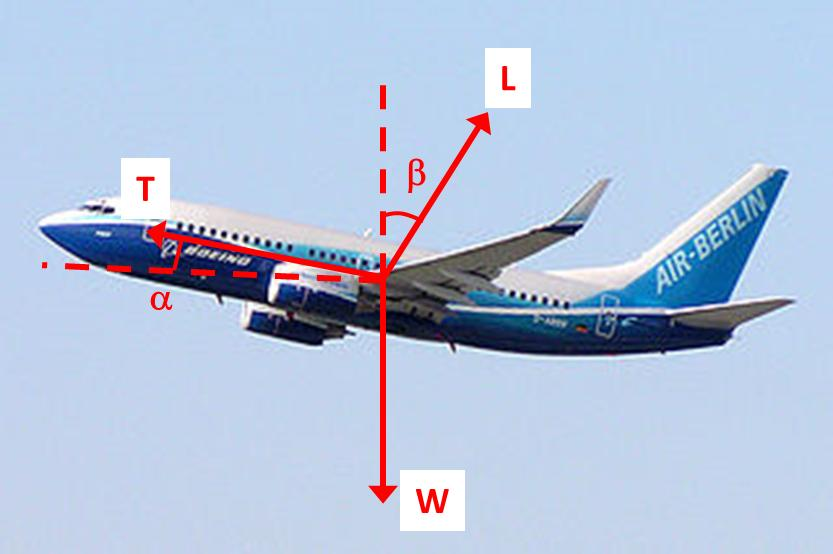
\includegraphics[height=1.8in]{boeing.jpg}
  \caption{Free-body Diagram of Boeing 737-700 (Photo due to Arcturus)}
\end{figure}

